% !TeX spellcheck = en_US
\chapter{Implementation and Validation}%

The first step of the validation involves constructing a basic model that captures the kinematics and dynamics of an industrial robot. To test the method in a simple case, the first tests are performed on a 6-DoF model with one redundant DoF. After validation on this simple model, additional redundant DoF are introduced. 

Once the basic mathematical model is established, various optimization algorithms are implemented to determine the optimal values for each parameter associated with the redundant DoF. These methods and optimization algorithms can consider the industrial robot's specific objectives and constraints, like energy consumption or joint accelerations. 

After that, the goal is to incorporate this method with a selected CAM software to be tested in more complex scenarios.

Further validation processes entails conducting real-world tests and simulations to evaluate optimized parameter performance and verify the effectiveness of the proposed methodology.
\section{Simple Implementation}%
To test the proposed method a 6-DoF robot is modeled. 

 \begin{figure}[H]
	\centerline{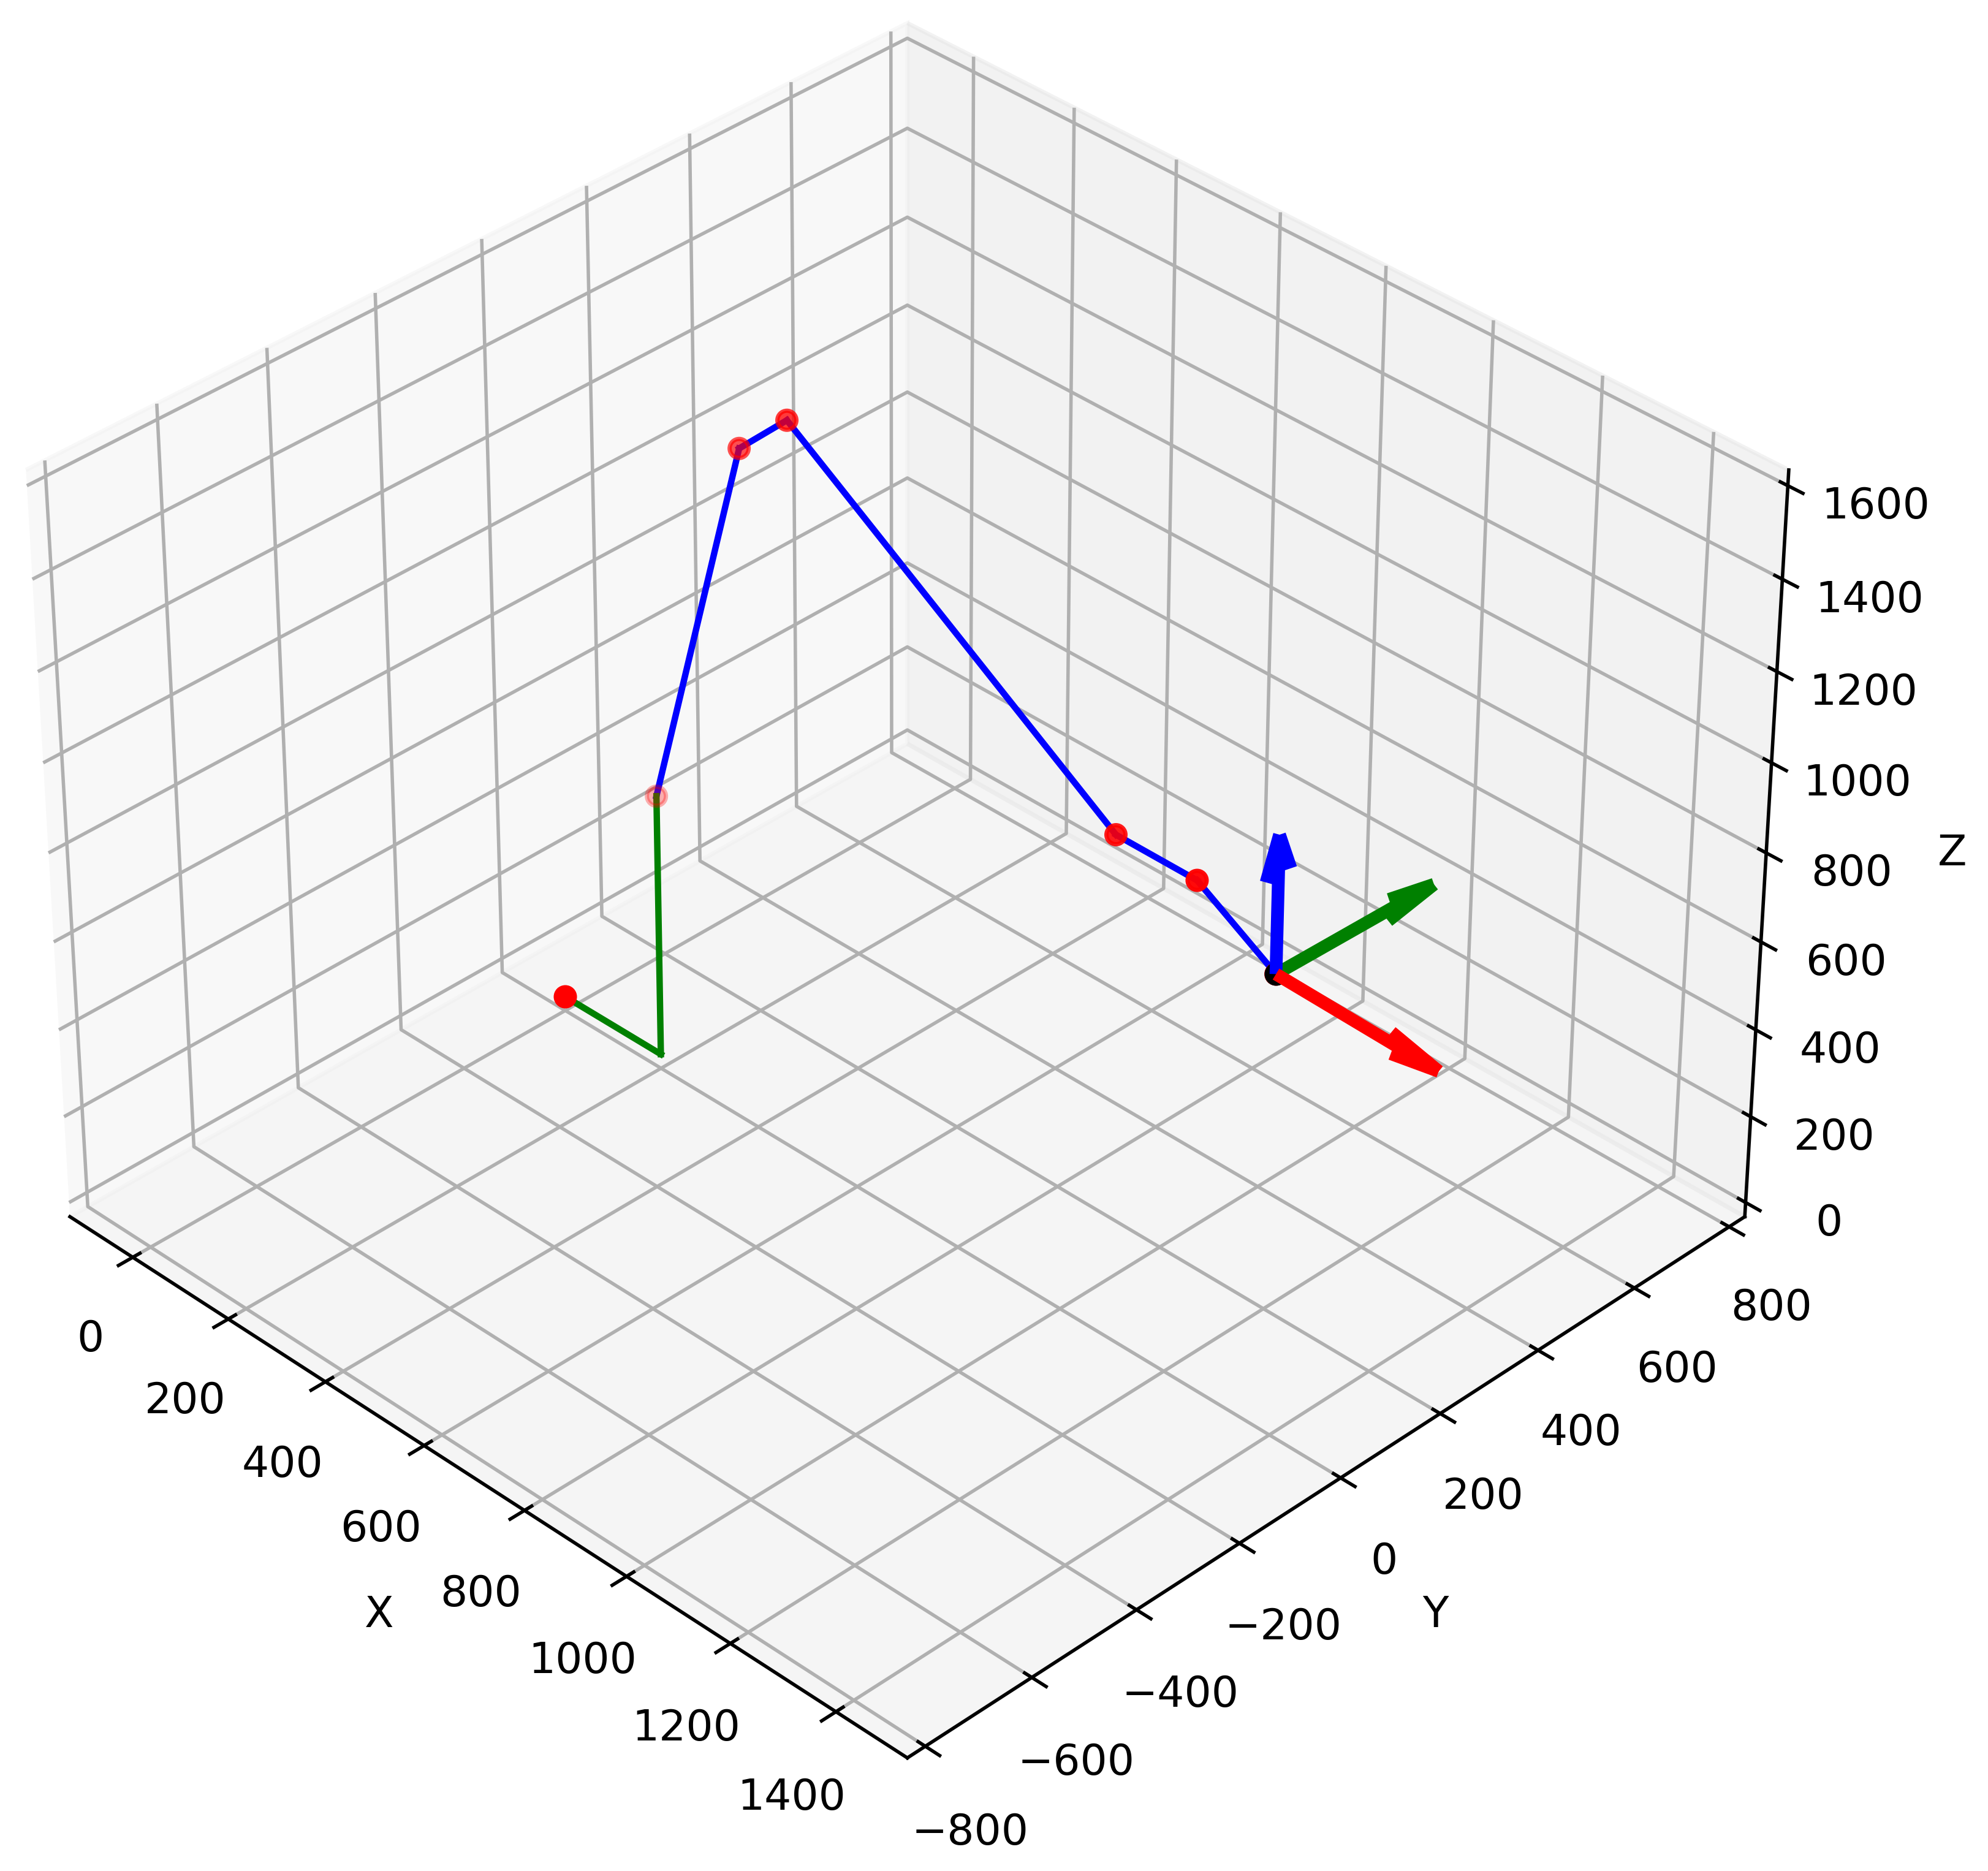
\includegraphics[width=0.9\textwidth]{figures/robotprog.png}}
	\caption{x}
	\label{robotprog}
\end{figure}
\section{Testing and Validation}%

\section{Analysis and Discussion of the results}%


\subsection{Analysis}
\subsection{Discussion}%